

%%%%% PREAMBLE %%%%%

\documentclass{article} % Gives you the type of document
\usepackage[margin=1in]{geometry} % Sets the size of the margins
\usepackage{parskip}	% This is to avoid indenting paragraphs and creates paragraph breaks by just hitting the enter key
\usepackage[T1]{fontenc}

%Tables preamble
\usepackage[none]{hyphenat} % Stops words from breaking up in tables
\usepackage{array}

%Math preamble
\usepackage{amsmath}

% Graphics preamble
\usepackage{graphicx}	% For importing images
\usepackage{float} 		% Allows for control of float positions 
\usepackage{caption} 
\usepackage{subcaption}
\captionsetup[table]{skip=10pt}

%Header and Footer preamble
\usepackage{fancyhdr}
\pagestyle{fancy}
\fancyhf{}	% 
%\fancyhead{}	% This command clears the header from the "fancy" page style
%\fancyfoot{}	% This command clears the footer from the "fancy" page style
%\fancyfoot[C]{ \thepage\ }	% This command inserts the page number on the right side of the footer
%\renewcommand{\headrulewidth}{0pt}	% Fancy page style adds horizontal lines between the header and footer
%\renewcommand{\headrulewidth}{0pt}	% These two commands removes those separation lines


%--------------------------------------------------------------------
%
% Header and Footer options
%
%--------------------------------------------------------------------
\lhead{\bfseries Robotics Analysis and Synthesis}
\chead{\bfseries Lab 06}
\rhead{Group 2}

%\lfoot{}\cfoot{\thepage}\rfoot{}

%---------------------------------------------------------------------
%
% DOCUMENT STARTS HERE 
%
%--------------------------------------------------------------------

\begin{document}
%--------------------------------------------------------------------
% Cover page of Lab report with group, dates, version info, etc.
%--------------------------------------------------------------------
\begin{titlepage}

	\begin{figure}
	\centering
	
\includegraphics[width=3in]{images/ksulogo2.png}  % Includes the KSU logo in the title page
	\end{figure}

	\title{MTRE 4200-01: Robotics Analysis and Synthesis\\ Lab 06: Simulated Robotic Arm} % Replace the \# with the lab number
	\date{Date of Experiment: February 28, 2023 \\ [2mm] Date Submitted via D2L: March 13, 2023 , Version 1}
	\author{}  % Replace the \# with your group number
	\maketitle
	\thispagestyle{empty} % This command eliminates the page number from the title page.  It clears the default style.

\end{titlepage}

%--------------------------------------------------------------------
%
% Header and Footer options
%
%--------------------------------------------------------------------

\lfoot{MTRE 4200}
\cfoot{Page \thepage}
\rfoot{\bfseries SPRING 2023}

%\lfoot{}\cfoot{\thepage}\rfoot{}

%--------------------------------------------------------------------
%\newpage 

%Table of contents and list of figures here

\tableofcontents



\setcounter{page}{1} % Setting the counter here will begin the page numbering on this page


%\newpage

%This is the main body of the lab report
% Member contributions

%--------------------------------------------------------------------
%
%%%%% MEMBERS %%%%%
%
%--------------------------------------------------------------------

\section{Member Contributions}
	
	\begin{itemize}
	\item Ben Hall
	\item Brighton Swales
	\item Sebastian Diaz Mora
	\item Ruben Murillo
	\end {itemize}

%--------------------------------------------------------------------
%
%%%%% ABSTRACT %%%%%
%
%--------------------------------------------------------------------

\section{Abstract} 

The Simulated Robotic Arm lab of ROS provides practical experience in working with robotic arms using the ROS framework. This lab covers creating a simulated robotic arm, controlling its movement using different algorithms, and visualizing data using ROS tools. The goal of this lab is to provide students with hands-on experience in developing ROS-based robotic arm systems.


\newpage 


\section{Results}

Here are the screenshots showcasing the results of the process of the Simulated Robotic Arm lab, where the student learned how to create a simulated robotic arm, control its movement using different algorithms and visualize data using ROS tools.
	
\begin{figure}[h]
	\centering
	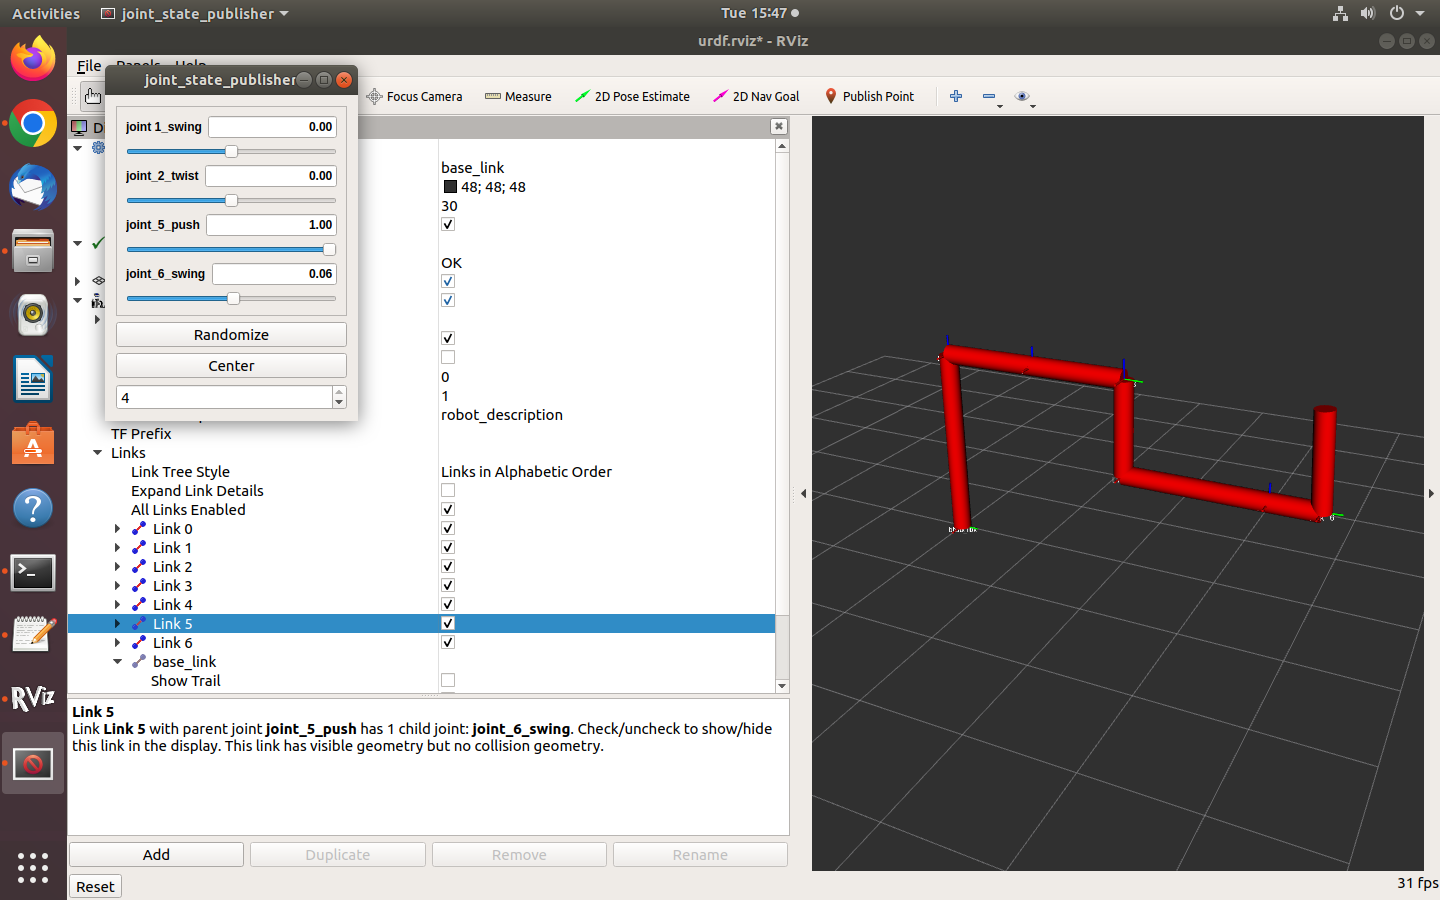
\includegraphics[width=0.8\textwidth]{images/ss3.png}
\end{figure}

\begin{figure}[h]
	\centering
	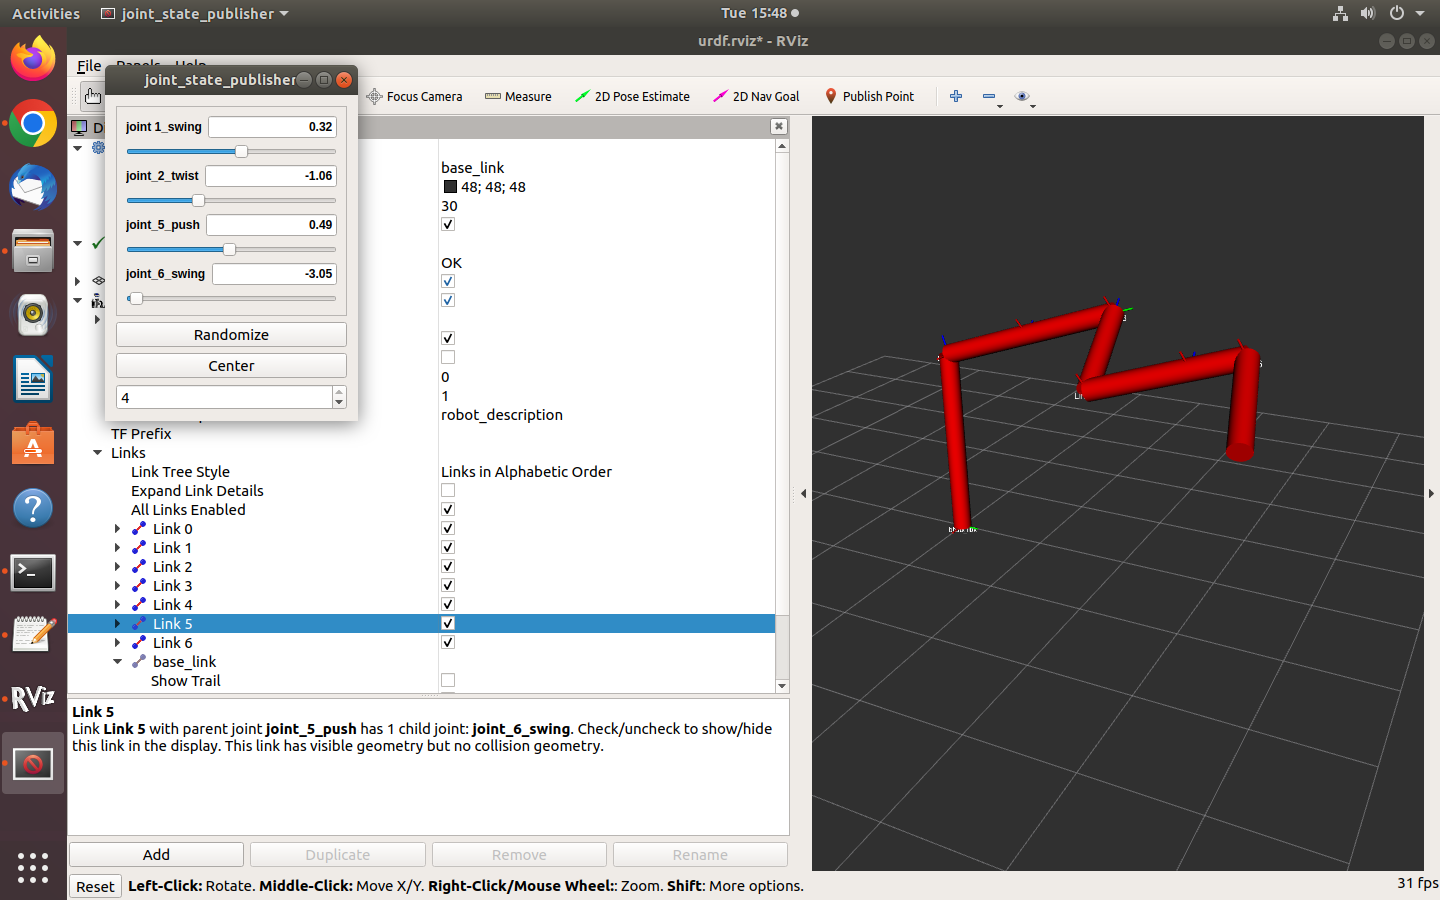
\includegraphics[width=0.8\textwidth]{images/ss4.png}
\end{figure}

\newpage

\begin{figure}[h]
	\centering
	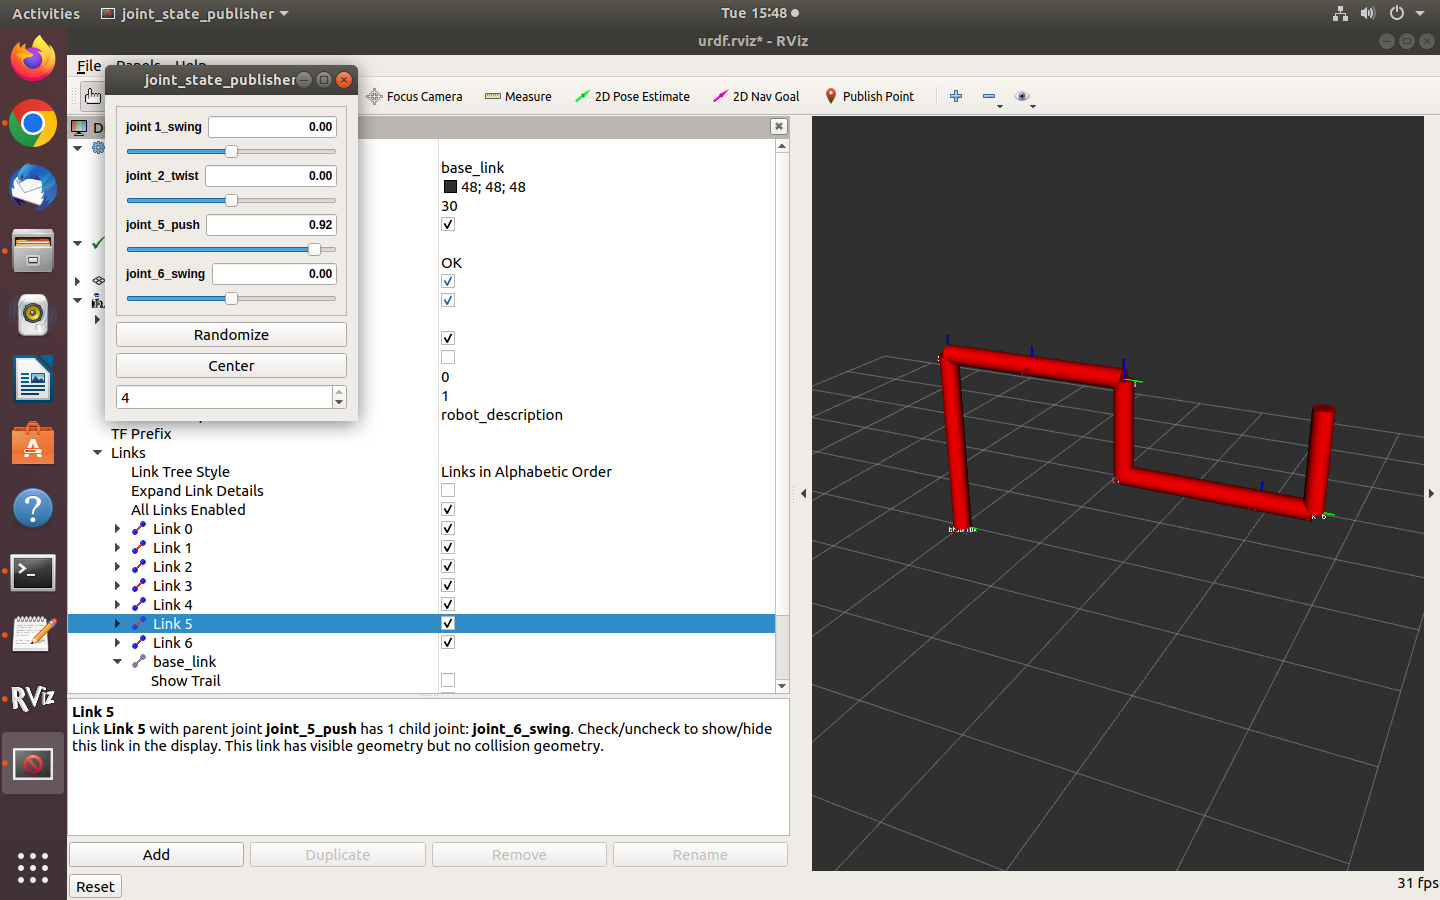
\includegraphics[width=0.8\textwidth]{images/ss5.png}
\end{figure}

\begin{figure}[h]
	\centering
	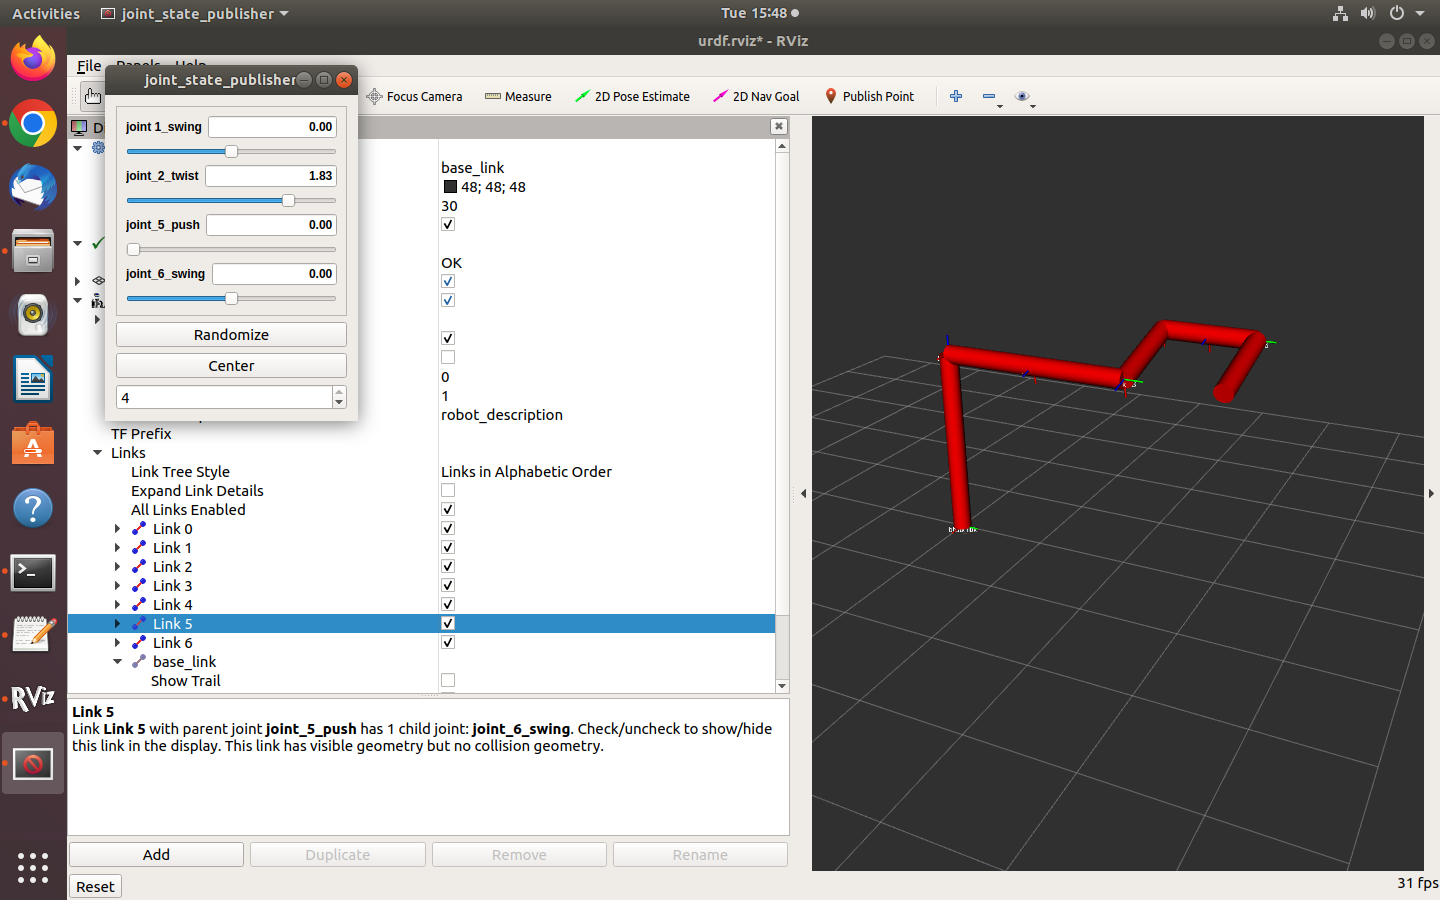
\includegraphics[width=0.8\textwidth]{images/ss6.png}
\end{figure}

\newpage

\begin{figure}[h]
	\centering
	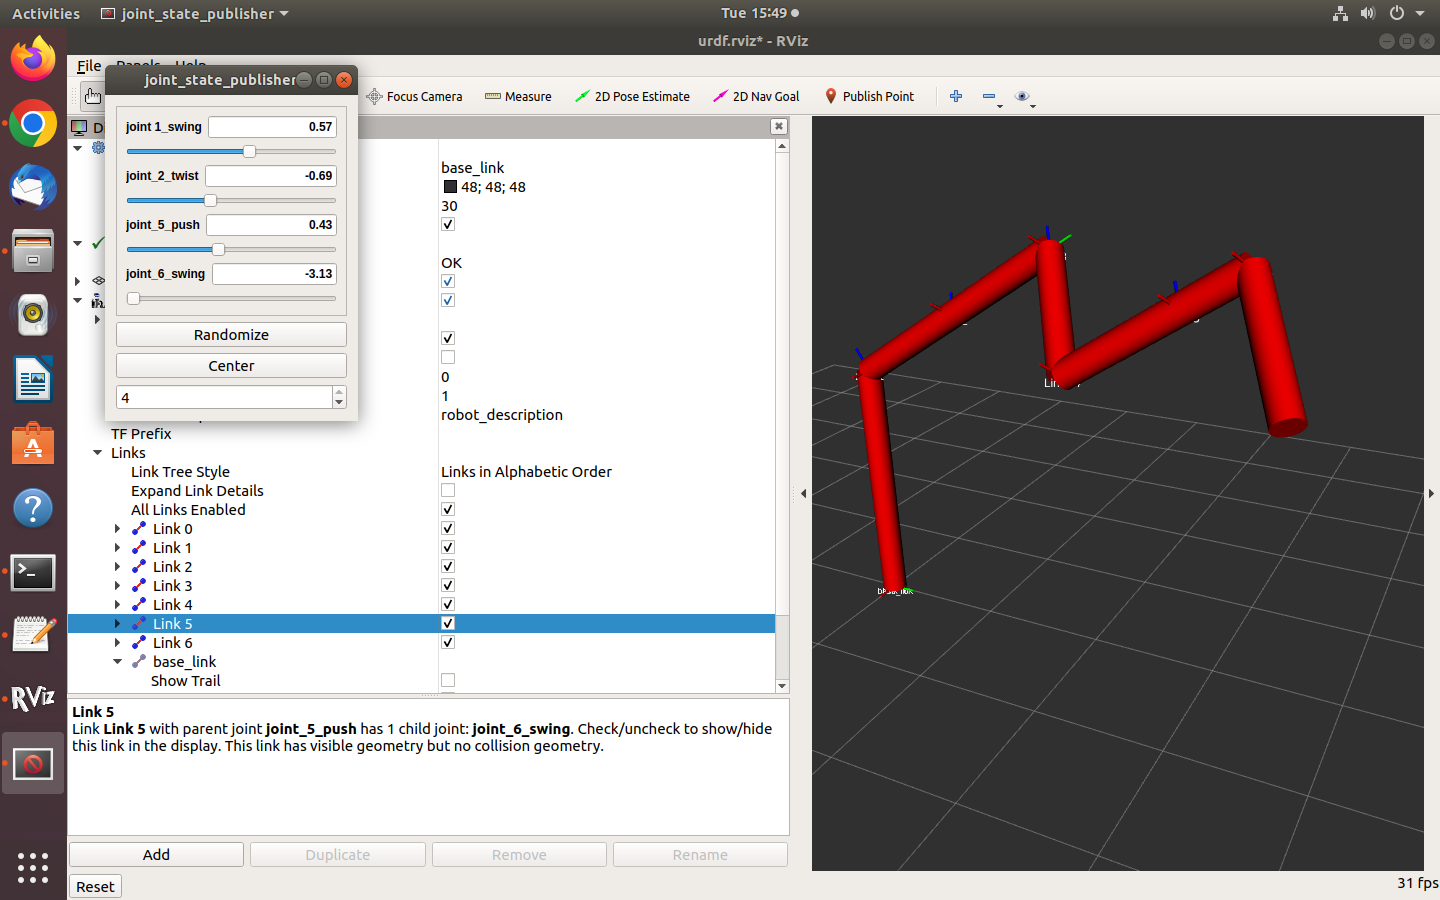
\includegraphics[width=0.8\textwidth]{images/ss7.png}
\end{figure}


\section{Conclusion}

The Simulated Robotic Arm lab of ROS provides practical knowledge in working with ROS-based robotic arm systems. This lab is essential for students who are interested in developing robotic arm systems using the ROS framework.




\end{document}

